% !TEX root = ../notes_unsupervisedlearning.tex
% Chapter 11: Self-Training and Ensemble Methods
%%%%%%%%%%%%%%%%%%%%%%%%%%%%%%%%%%%%%%%%%%%%%%%%%%%%%%%%%%%%%%%%%%%%%%

\chapter{Self-Training and Ensemble Methods}\index{Self-Training}\index{Pseudo-Labeling}\index{FixMatch}
\newthought{The model becomes the teacher.}

%═══════════════════════════════════════════════════════════════════════
% BLOCK 1: INTRODUCTION
%═══════════════════════════════════════════════════════════════════════

\section{The Why}

\marginnote{Conditional independence plus agreement suggests truth.}

You have a small labelled dataset and a large unlabelled one. Can the model leverage the unlabelled data to improve?

\newthought{Self-training}\index{self-training} uses the model's own predictions on unlabelled data as additional training signal. The key insight: if the model is confident about an unlabelled example, that prediction is likely correct.

\newthought{Semi-supervised learning}\index{semi-supervised learning} combines labelled and unlabelled data. Labelled data provides ground truth, unlabelled data reveals data structure, and self-training bridges the two.

\newthought{In order to move from scarce labels to leveraging abundant unlabelled data} we have good reason to find ways to,
\begin{itemize}
    \item use confident model predictions as pseudo-labels to expand the training set without human annotation.
    \item enforce prediction consistency under augmentation so that the model learns representations that are stable to input perturbations.
    \item combine multiple views or models to reduce the risk of confirmation bias in self-generated labels.
\end{itemize}

\subsection{Hands On Experience}

\begin{marginfigure}
\begin{tikzpicture}[scale=0.7]
    \begin{axis}[
        xlabel={$x_1$}, ylabel={$x_2$},
        xmin=0, xmax=10, ymin=0, ymax=10,
        width=\textwidth, height=\textwidth,
        axis line style={draw=none},
        tick style={black, thin},
        tick align=outside, tick pos=left,
        xtick={2,4,6,8}, ytick={2,4,6,8},
        xticklabel style={font=\tiny},
        yticklabel style={font=\tiny},
    ]
    % Labeled points
    \addplot[only marks, mark=*, mark size=3pt, black] coordinates {(2,2) (3,3)};
    \addplot[only marks, mark=*, mark size=3pt, black!55] coordinates {(7,7) (8,8)};
    % Unlabeled points
    \addplot[only marks, mark=o, mark size=2pt, black!30] coordinates {
        (2.5,2.5) (1.5,2) (3,2) (2,3)
        (7.5,7.5) (6.5,7) (8,7) (7,8)
        (5,5)
    };
    \end{axis}
\end{tikzpicture}
\caption{Few labelled points (filled), many unlabelled (hollow). Self-training expands labels iteratively.}
\label{fig:self_training_intro}
\end{marginfigure}

Start with 2 labelled points per class. Train a classifier. Which unlabelled points would you confidently label? Add them to the training set and repeat.

\newthought{The Learning Objectives} of this lecture:
\begin{itemize}
    \item Implement pseudo-labelling with confidence thresholding and explain how confirmation bias arises and compounds.
    \item Apply consistency regularisation and the FixMatch framework to combine pseudo-labels with strong augmentation.
    \item Design multi-view learning with co-training and identify when the conditional independence assumption holds.
\end{itemize}

%═══════════════════════════════════════════════════════════════════════
% BLOCK 2: MAIN THEORY
%═══════════════════════════════════════════════════════════════════════

\newpage
\section{Pseudo-Labeling}\index{pseudo-labeling}

\marginnote{Use confident predictions as if they were ground truth~\cite{Lee2013PseudoLabel}.}

\begin{algorithm}[H]
\caption{Basic Pseudo-Labeling}
\begin{algorithmic}[1]
\Require Labeled set $\mathcal{L}$, unlabeled set $\mathcal{U}$, threshold $\tau$
\State Train model $f$ on $\mathcal{L}$
\Repeat
    \For{each $x \in \mathcal{U}$}
        \State $\hat{p} \gets f(x)$, $\hat{y} \gets \arg\max \hat{p}$
        \If{$\max(\hat{p}) > \tau$}
            \State Add $(x, \hat{y})$ to $\mathcal{L}$
            \State Remove $x$ from $\mathcal{U}$
        \EndIf
    \EndFor
    \State Retrain $f$ on expanded $\mathcal{L}$
\Until{convergence or $\mathcal{U}$ empty}
\end{algorithmic}
\end{algorithm}

\newthought{Key design choices:}
\begin{itemize}
    \item Threshold $\tau$: higher values yield fewer but more accurate pseudo-labels
    \item Curriculum: start with a high threshold, gradually lower it
    \item Soft vs.\ hard: use soft labels $\hat{p}$ or hard labels $\hat{y}$
\end{itemize}


\section{Confidence Thresholding}\index{confidence thresholding}

\marginnote{High confidence does not guarantee correctness, but the two are correlated.}

\subsection{The Problem}

\newthought{Neural networks are often overconfident,} especially on out-of-distribution data, when trained on small datasets, and near decision boundaries.

\subsection{Calibration}\index{calibration}

\newthought{A well-calibrated model} satisfies $P(\hat{y} = y | \hat{p} = p) = p$. Temperature scaling adjusts logits: $\hat{p}_{\text{calibrated}} = \text{softmax}(z / T)$ with $T > 1$ typically.

\subsection{Confirmation Bias}\index{confirmation bias}

\marginnote{Errors in pseudo-labels get reinforced in a dangerous feedback loop.}

\newthought{Self-training can amplify mistakes:} the model makes an error on an unlabelled point, that error becomes a pseudo-label, the model trains on the wrong label, and the model becomes more confident in the error. Mitigation strategies include high thresholds, curriculum scheduling, and using multiple models.


\section{Consistency Regularization}\index{consistency regularization}

\marginnote{Predictions should be stable under perturbation.}

\newthought{The key assumption} is that small perturbations should not change the class:

\begin{equation}
    \mathcal{L}_{\text{consistency}} = \sum_{x \in \mathcal{U}} d(f(x), f(\text{aug}(x)))
\end{equation}

where $\text{aug}$ applies data augmentation and $d$ is a distance such as MSE or KL divergence.

\subsection{Mean Teacher}\index{Mean Teacher}

\newthought{Mean Teacher} uses an exponential moving average of model parameters as teacher~\cite{Tarvainen2017MeanTeacher}:

\begin{equation}
    \theta_{\text{teacher}} \gets \alpha \theta_{\text{teacher}} + (1 - \alpha) \theta_{\text{student}}
\end{equation}

\begin{figure}
\centering
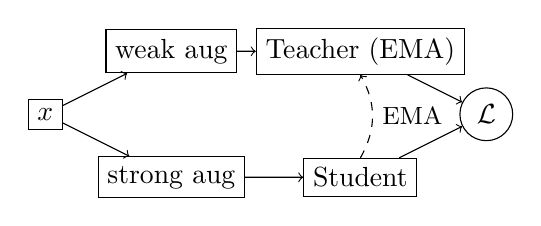
\begin{tikzpicture}[scale=0.8]
    \node[draw, rectangle] (x) at (0,0) {$x$};
    \node[draw, rectangle] (aug1) at (2,1) {weak aug};
    \node[draw, rectangle] (aug2) at (2,-1) {strong aug};
    \node[draw, rectangle] (teacher) at (5,1) {Teacher (EMA)};
    \node[draw, rectangle] (student) at (5,-1) {Student};
    \node[draw, circle] (loss) at (7,0) {$\mathcal{L}$};

    \draw[->] (x) -- (aug1);
    \draw[->] (x) -- (aug2);
    \draw[->] (aug1) -- (teacher);
    \draw[->] (aug2) -- (student);
    \draw[->] (teacher) -- (loss);
    \draw[->] (student) -- (loss);
    \draw[->, dashed] (student.north) to[bend right] node[right] {\small EMA} (teacher.south);
\end{tikzpicture}
\caption{Mean Teacher: student learns to match the EMA teacher's predictions.}
\label{fig:mean_teacher}
\end{figure}


\section{Co-Training and Multi-View Learning}\index{co-training}

\marginnote{Multiple views provide independent supervision.}

\subsection{Co-Training}

\newthought{Co-training} assumes features split into two conditionally independent views given the label~\cite{Blum1998CoTraining}:

\begin{algorithm}[H]
\caption{Co-Training}
\begin{algorithmic}[1]
\State Train classifier $f_1$ on view 1 features
\State Train classifier $f_2$ on view 2 features
\Repeat
    \State $f_1$ labels high-confidence unlabeled points
    \State Add to $f_2$'s training set
    \State $f_2$ labels high-confidence unlabeled points
    \State Add to $f_1$'s training set
    \State Retrain both classifiers
\Until{convergence}
\end{algorithmic}
\end{algorithm}

\newthought{Example views:} for web pages, view 1 is page content and view 2 is anchor text from links.

\subsection{Tri-Training}

\newthought{Tri-training} uses three classifiers; a point is labelled for $f_3$ if $f_1$ and $f_2$ agree:
\begin{equation}
    \text{Pseudo-label } x \text{ for } f_3 \text{ if } f_1(x) = f_2(x)
\end{equation}


\section{FixMatch}\index{FixMatch}

\marginnote{\newthought{FixMatch.} State-of-the-art semi-supervised learning~\cite{Sohn2020FixMatch}.}

\newthought{FixMatch} combines pseudo-labelling and consistency:

\begin{enumerate}
    \item Apply weak augmentation such as flip and crop
    \item Generate pseudo-label if confidence exceeds $\tau$
    \item Apply strong augmentation such as RandAugment or CTAugment
    \item Train to match pseudo-label on the strongly augmented view
\end{enumerate}

\begin{equation}
    \mathcal{L} = \mathcal{L}_{\text{supervised}} + \lambda \sum_{x \in \mathcal{U}} \mathbf{1}[\max(\hat{p}) > \tau] \cdot H(\hat{y}, f(x_{\text{strong}}))
\end{equation}

\begin{figure}
\centering
\begin{tikzpicture}[scale=0.7]
    \node[draw, rectangle] (x) at (0,0) {Unlabeled $x$};
    \node[draw, rectangle] (weak) at (3,1.5) {Weak aug};
    \node[draw, rectangle] (strong) at (3,-1.5) {Strong aug};
    \node[draw, rectangle] (model1) at (6,1.5) {Model};
    \node[draw, rectangle] (model2) at (6,-1.5) {Model};
    \node[draw, diamond, aspect=2] (check) at (9,1.5) {$> \tau$?};
    \node[draw, rectangle] (pseudo) at (9,0) {Pseudo-label};
    \node[draw, circle] (loss) at (9,-1.5) {CE Loss};

    \draw[->] (x) -- (weak);
    \draw[->] (x) -- (strong);
    \draw[->] (weak) -- (model1);
    \draw[->] (strong) -- (model2);
    \draw[->] (model1) -- (check);
    \draw[->] (check) -- node[right] {yes} (pseudo);
    \draw[->] (pseudo) -- (loss);
    \draw[->] (model2) -- (loss);
\end{tikzpicture}
\caption{FixMatch: pseudo-labels from weak augmentation train predictions on strong augmentation.}
\label{fig:fixmatch}
\end{figure}


\section{Model-in-the-Loop Labeling}

\marginnote{Large models generate candidates; humans verify.}

\newthought{The key insight} is that it is easier to verify than to create. A foundation model generates candidate labels, a human reviews and corrects them, and the process is much faster than labelling from scratch.

\newthought{Applications} include GPT generating NER annotations for review, SAM proposing segmentation masks for correction, and CLIP classifying images with humans fixing errors.


%═══════════════════════════════════════════════════════════════════════
% BLOCK 3: STUDENT ACTIVATION
%═══════════════════════════════════════════════════════════════════════

\newpage
\section{Examples \& Exercises}

\subsection{Exercise 1: Pseudo-Labeling Threshold}

You have 100 unlabelled points. Model confidence distribution:
\begin{itemize}
    \item 20 points with confidence $> 0.95$, of which 18 are correct
    \item 30 points with confidence 0.8--0.95, of which 21 are correct
    \item 50 points with confidence $< 0.8$, of which 25 are correct
\end{itemize}

\begin{enumerate}
    \item What is the pseudo-label accuracy at $\tau = 0.95$?
    \item At $\tau = 0.8$?
    \item What threshold would you choose, and why?
\end{enumerate}

\subsection{Exercise 2: Confirmation Bias}

A model repeatedly misclassifies ironic positive reviews as negative. Explain how self-training makes this worse.

\subsection{Exercise 3: FixMatch Design}

Why use weak augmentation for pseudo-labels but strong augmentation for training?


\section{Self-Reflection and Recap}

\newthought{Self-Reflection.}

\begin{enumerate}
    \item Why might pseudo-labelling fail on imbalanced data?
    \item How does FixMatch mitigate confirmation bias compared to basic pseudo-labelling?
    \item When does the conditional independence assumption in co-training hold, and when does it break?
    \item What is the relationship between temperature scaling and the pseudo-label threshold $\tau$?
    \item How does the Mean Teacher's EMA update stabilise training compared to a static teacher?
    \item Why is strong augmentation essential for the consistency regularisation to be useful?
    \item What failure mode arises when the initial labelled set is too small or unrepresentative?
\end{enumerate}

\vspace{1.5em}

\newthought{Recap.}

\begin{itemize}
    \item Pseudo-labelling uses confident model predictions as training signal; confirmation bias is the central failure mode, where errors reinforce themselves.
    \item Consistency regularisation forces predictions to be stable under augmentation, providing a complementary training signal from unlabelled data.
    \item Co-training exploits conditionally independent views so that each classifier labels data for the other, reducing shared errors.
    \item FixMatch combines pseudo-labels from weak augmentation with training on strong augmentation, achieving state-of-the-art semi-supervised performance with a simple framework.
\end{itemize}

\vspace{2.5em}

\marginnote{\newthought{Teaser.} Self-training uses the model's predictions, but sometimes we need human guidance during training, not just at the start.}

\newthought{Self-training treats the model as its own teacher.} But the model can only teach what it already knows, and its mistakes compound. Some problems require a human in the loop: correcting predictions, selecting informative examples to label, or demonstrating the desired behaviour.

\newthought{The next chapter explores interactive and imitation learning,} where active learning queries the most informative examples, behaviour cloning learns from demonstrations, and DAgger addresses the covariate shift that makes naive imitation brittle.

\marginnote{\newthought{feedback}}
